 \documentclass[a4paper,12pt,brazil,doubleside]{book}

% tentei incluir o da pasta comum mas não funcionou
% \usepackage{amssymb}                        %%% para simbolo de 'marca registrada'
\usepackage[brazil]{varioref}               %%% referencias com página \vref
\usepackage[sf,bf,compact,topmarks,calcwidth,pagestyles]{titlesec} %%% definir títulos de seção
\usepackage{amsmath,amsfonts,amstext,amsthm,textcomp}
\usepackage{fancybox}                       %%% boxes
\usepackage[dvipsnames,usenames]{color}                          %%% Cores de fonte e fundo
\usepackage[dvipsnames,usenames]{xcolor}
\usepackage{colortbl}                       %%% Cores em tabelas
\usepackage{rotating}
\usepackage{fancyvrb}                       %%% Inclusão de texto usando VerbatimInput
\usepackage{bookman}                        %%% Fonte de Letras
\usepackage{enumerate}
\usepackage{lettrine}
\usepackage{minted}	
\usepackage{caption}
\usepackage{framed}
\usepackage{enumitem}

%\usepackage{listings}
%\lstset{
%  numbers=left,
%  numberstyle=\tiny,
%  mathescape=true,
%  frame=single,
%  stepnumber=1,
%%  basicstyle=\scriptsize, % fontes menores nos codigos
%  keywordstyle=\ttfamily,
%  identifierstyle=\ttfamily, % \bfseries negrito nos codigos
%  commentstyle=\ttfamily
%}
\usepackage{pstricks} % listings color: black!50!red

\usepackage{listings}
\lstset{
	numbers=left,
	stepnumber=1,
	firstnumber=1,
	numberstyle=\tiny,
	mathescape=true,
	extendedchars=true,
	breaklines=true,
	frame=single,
	basicstyle=\footnotesize,
%	basicstyle=\scriptsize,
	stringstyle=\ttfamily,
% 	moredelim=*[l][\itshape]{||},%
	showstringspaces=false,
	float=h,
}
\lstdefinelanguage{lalp} {
  sensitive=true,
  keywordstyle={\color{black!50!green}\ttfamily\bfseries},
  keywords={const, typedef, fixed, in, out, counter, when, block_ram, delay_op, mult_op_s, add_reg_op_s},
  otherkeywords={<-},
  otherkeywords={@},
  commentstyle={\color{black!50!red}\itshape},
  morecomment=[l]{//}, 
  morecomment=[s]{/*}{*/},
}
\lstdefinelanguage{ican} {
  sensitive=true,
  keywordstyle={\color{black!50!red}\ttfamily\bfseries},
  keywords={array, begin, boolean, by, case, character, default, do, each, elif, else, end, enum, esac, false, fi, for, goto, if, in, inout, integer, nil, od, of, out, procedure, real, record, repeat, return, returns, sequence, set, to, true, until, where, while},
  commentstyle={\color{black!50!green}\itshape},
  morecomment=[l]{||},
  literate={{(X)}{$\times$}1 {(E)}{$\in$}1 {(U)}{$\cup$}1 {(N)}{$\cap$}1 {(<)}{$\langle$}1 {(>)}{$\rangle$}1 {->}{$\rightarrow$}2 {<\-}{$\leftarrow$}2 {=}{$=$}1 {>}{$>$}1 {<}{$<$}1 {!=}{$\neq$}1 {>=}{$\ge$}1 {<=}{$\le$}1}
}

\renewcommand\listingscaption{Algoritmo}
\renewcommand\listoflistingscaption{Lista de Algoritmos}


\usepackage[english,brazil]{babel}
\usepackage[utf8]{inputenc}
\usepackage[T1]{fontenc}
\usepackage{times}
\usepackage{graphicx,xr}
\usepackage{subfigure}
\usepackage{longtable}
\usepackage{setspace}
\usepackage{multirow}
\usepackage{rotating}
\usepackage{indentfirst}
\usepackage{xspace}
\usepackage[sort]{natbib}
\usepackage[a4paper,top=30mm,bottom=20mm,left=30mm,right=20mm]{geometry}

\usepackage{hyperref}
\hypersetup{
%  backref, %omitir na versão final
  pdfsubject =	{...},
  pdftitle =	{...},
  pdfkeywords = {...},
  pdfauthor =	{Ricardo Menotti, Daniel Lucrédio, ...},
  colorlinks =	{true}, %true na versão final
  linkcolor =	{black!50!blue},
  citecolor =	{black!50!blue},
  urlcolor =	{black!50!blue},
}

\exhyphenpenalty = 10000

\onehalfspace

\hyphenation{es-ta-be-le-ci-das a-tu-al-men-te Simple-Scalar-ARM}

\newcommand{\up}[1]{\raisebox{1.5ex}[0pt]{#1}}

\newcommand{\bi}{\begin{itemize}}
\newcommand{\ei}{\end{itemize}}
\newcommand{\be}{\begin{enumerate}}
\newcommand{\ee}{\end{enumerate}}

\definecolor{Gray}{gray}{0.9}

% using \autoref{} instead
%\newcommand{\reffig}[1]{Figura~\ref{fig:#1}}
%\newcommand{\reftab}[1]{Tabela~\ref{tab:#1}}
%\newcommand{\refcha}[1]{Capítulo~\ref{cha:#1}}
%\newcommand{\refses}[1]{Seção~\ref{ses:#1}}
%\newcommand{\refsub}[1]{Subseção~\ref{sub:#1}}
%\newcommand{\refape}[1]{Apêndice~\ref{ape:#1}}
%\newcommand{\refcod}[1]{Código~\ref{cod:#1}}
\newcommand{\subfigureautorefname}{\figureautorefname}

\newcommand{\cha}[2]{\chapter{#2}\label{cha:#1}} %\thispagestyle{empty}
\newcommand{\ses}[2]{\section{#2}\label{ses:#1}}
\newcommand{\sub}[2]{\subsection{#2}\label{sub:#1}}
\newcommand{\ape}[2]{\chapter{#2}\label{ape:#1}} %\thispagestyle{empty}

\newcommand{\figsim}[2]{
\begin{figure}[!ht]
  \centering
  \includegraphics[width=\textwidth]{../figuras/#1.jpg}
  \caption{#2}
  \label{fig:#1}
\end{figure}
}

\newcommand{\ew}[1]{\selectlanguage{english}\emph{#1}\selectlanguage{brazil}}
%\newcommand{\ew}[1]{\emph{#1}}

\renewcommand{\bibname}{Referências Bibliográficas}

\setcounter{secnumdepth}{2}

\setcounter{tocdepth}{2}

\pagestyle{empty}

%\font\numberfont= goxi2074 scaled 2000      %%% Fonte para o Número do Capítulo
\font\numberfont= pzcmi scaled 6500      %%% Fonte para o Número do Capítulo

                                            %%% redefine o formato do título
\titleformat{\chapter}[display]
  {\normalfont\Large\sffamily
  }
  {
   \rule[32pt]{.7\linewidth}{4pt}
   \hspace{-10pt}
   \shadowbox{
   \begin{minipage}{.18\linewidth}
     \begin{center}
       \textsc{\Large\chaptertitlename}\\
       \vspace{1ex}
       {\numberfont \thechapter}\\
       \vspace{1ex}
     \end{center}
   \end{minipage}}
  }
  {0pt}
  {\filcenter
   \Huge
   }
  [\hfill\rule{.8\textwidth}{0.75pt}\\
     \vskip-1.8ex\hfill\rule{.7\textwidth}{2pt}]


\newpagestyle{body}{ %[\small\sffamily]{
\headrule

\sethead[\thepage][][\ifthechapter{\thechapter\quad}{} \textsl{\chaptertitle}]%
          {\ifthechapter{\thechapter\quad \textsl{\chaptertitle}}{\textsl{\chaptertitle}}}{}{\thepage}


}

\newpagestyle{misc}{
  \headrule
  \sethead{\textsl{\chaptertitle}}{}{\thepage}
  \setfoot{}{}{}
}

\font\largefont= pzcmi scaled 6500

\newcommand{\versal}[1]{{\noindent
    \setbox0\hbox{\largefont #1 }%
    \count0=\ht0                   % height of versal
    \count1=\baselineskip          % baselineskip
    \divide\count0 by \count1      % versal height/baselineskip
    \dimen1 = \count0\baselineskip % distance to drop versal
    \advance\count0 by 1\relax     % no of indented lines
    \dimen0=\wd0                   % width of versal
    \global\hangindent\dimen0      % set indentation distance
    \global\hangafter-\count0      % set no of indented lines
    \hskip-\dimen0\setbox0\hbox to\dimen0{\raise-\dimen1\box0\hss}%
    \dp0=0in\ht0=0in\box0}}


%%%  define linha mais grossa para tabelas

\newdimen\arrayruleHwidth
\setlength{\arrayruleHwidth}{2pt} \makeatletter
\def\Hline{\noalign{\ifnum0=`}\fi\hrule \@height \arrayruleHwidth
\futurelet \@tempa\@xhline} \makeatother

\definecolor{mygreen}{rgb}{0.1, 0.6, 0.2}

\usepackage{amssymb}                        %%% para simbolo de 'marca registrada'
\usepackage[brazil]{varioref}               %%% referencias com página \vref
\usepackage[sf,bf,compact,topmarks,calcwidth,pagestyles]{titlesec} %%% definir títulos de seção
\usepackage{amsmath,amsfonts,amstext,amsthm,textcomp}
\usepackage{fancybox}                       %%% boxes
\usepackage[dvipsnames,usenames]{color}                          %%% Cores de fonte e fundo
\usepackage[dvipsnames,usenames]{xcolor}
\usepackage{colortbl}                       %%% Cores em tabelas
\usepackage{rotating}
\usepackage{fancyvrb}                       %%% Inclusão de texto usando VerbatimInput
\usepackage{bookman}                        %%% Fonte de Letras
\usepackage{enumerate}
\usepackage{lettrine}
\usepackage{minted}	
\usepackage{caption}
\usepackage{framed}
\usepackage{enumitem}

%\usepackage{listings}
%\lstset{
%  numbers=left,
%  numberstyle=\tiny,
%  mathescape=true,
%  frame=single,
%  stepnumber=1,
%%  basicstyle=\scriptsize, % fontes menores nos codigos
%  keywordstyle=\ttfamily,
%  identifierstyle=\ttfamily, % \bfseries negrito nos codigos
%  commentstyle=\ttfamily
%}
\usepackage{pstricks} % listings color: black!50!red

\usepackage{listings}
\lstset{
	numbers=left,
	stepnumber=1,
	firstnumber=1,
	numberstyle=\tiny,
	mathescape=true,
	extendedchars=true,
	breaklines=true,
	frame=single,
	basicstyle=\footnotesize,
%	basicstyle=\scriptsize,
	stringstyle=\ttfamily,
% 	moredelim=*[l][\itshape]{||},%
	showstringspaces=false,
	float=h,
}
\lstdefinelanguage{lalp} {
  sensitive=true,
  keywordstyle={\color{black!50!green}\ttfamily\bfseries},
  keywords={const, typedef, fixed, in, out, counter, when, block_ram, delay_op, mult_op_s, add_reg_op_s},
  otherkeywords={<-},
  otherkeywords={@},
  commentstyle={\color{black!50!red}\itshape},
  morecomment=[l]{//}, 
  morecomment=[s]{/*}{*/},
}
\lstdefinelanguage{ican} {
  sensitive=true,
  keywordstyle={\color{black!50!red}\ttfamily\bfseries},
  keywords={array, begin, boolean, by, case, character, default, do, each, elif, else, end, enum, esac, false, fi, for, goto, if, in, inout, integer, nil, od, of, out, procedure, real, record, repeat, return, returns, sequence, set, to, true, until, where, while},
  commentstyle={\color{black!50!green}\itshape},
  morecomment=[l]{||},
  literate={{(X)}{$\times$}1 {(E)}{$\in$}1 {(U)}{$\cup$}1 {(N)}{$\cap$}1 {(<)}{$\langle$}1 {(>)}{$\rangle$}1 {->}{$\rightarrow$}2 {<\-}{$\leftarrow$}2 {=}{$=$}1 {>}{$>$}1 {<}{$<$}1 {!=}{$\neq$}1 {>=}{$\ge$}1 {<=}{$\le$}1}
}

\renewcommand\listingscaption{Algoritmo}
\renewcommand\listoflistingscaption{Lista de Algoritmos}


\usepackage[english,brazil]{babel}
\usepackage[utf8]{inputenc}
\usepackage[T1]{fontenc}
\usepackage{times}
\usepackage{graphicx,xr}
\usepackage{subfigure}
\usepackage{longtable}
\usepackage{setspace}
\usepackage{multirow}
\usepackage{rotating}
\usepackage{indentfirst}
\usepackage{xspace}
\usepackage[sort]{natbib}
\usepackage[a4paper,top=30mm,bottom=20mm,left=30mm,right=20mm]{geometry}

\usepackage{hyperref}
\hypersetup{
%  backref, %omitir na versão final
  pdfsubject =	{...},
  pdftitle =	{...},
  pdfkeywords = {...},
  pdfauthor =	{Ricardo Menotti, Daniel Lucrédio, ...},
  colorlinks =	{true}, %true na versão final
  linkcolor =	{black!50!blue},
  citecolor =	{black!50!blue},
  urlcolor =	{black!50!blue},
}

\exhyphenpenalty = 10000

\onehalfspace

\hyphenation{es-ta-be-le-ci-das a-tu-al-men-te Simple-Scalar-ARM}

\newcommand{\up}[1]{\raisebox{1.5ex}[0pt]{#1}}

\newcommand{\bi}{\begin{itemize}}
\newcommand{\ei}{\end{itemize}}
\newcommand{\be}{\begin{enumerate}}
\newcommand{\ee}{\end{enumerate}}

\definecolor{Gray}{gray}{0.9}

% using \autoref{} instead
%\newcommand{\reffig}[1]{Figura~\ref{fig:#1}}
%\newcommand{\reftab}[1]{Tabela~\ref{tab:#1}}
%\newcommand{\refcha}[1]{Capítulo~\ref{cha:#1}}
%\newcommand{\refses}[1]{Seção~\ref{ses:#1}}
%\newcommand{\refsub}[1]{Subseção~\ref{sub:#1}}
%\newcommand{\refape}[1]{Apêndice~\ref{ape:#1}}
%\newcommand{\refcod}[1]{Código~\ref{cod:#1}}
\newcommand{\subfigureautorefname}{\figureautorefname}

\newcommand{\cha}[2]{\chapter{#2}\label{cha:#1}} %\thispagestyle{empty}
\newcommand{\ses}[2]{\section{#2}\label{ses:#1}}
\newcommand{\sub}[2]{\subsection{#2}\label{sub:#1}}
\newcommand{\ape}[2]{\chapter{#2}\label{ape:#1}} %\thispagestyle{empty}

\newcommand{\figsim}[2]{
\begin{figure}[!ht]
  \centering
  \includegraphics[width=\textwidth]{../figuras/#1.jpg}
  \caption{#2}
  \label{fig:#1}
\end{figure}
}

\newcommand{\ew}[1]{\selectlanguage{english}\emph{#1}\selectlanguage{brazil}}
%\newcommand{\ew}[1]{\emph{#1}}

\renewcommand{\bibname}{Referências Bibliográficas}

\setcounter{secnumdepth}{2}

\setcounter{tocdepth}{2}

\pagestyle{empty}

%\font\numberfont= goxi2074 scaled 2000      %%% Fonte para o Número do Capítulo
\font\numberfont= pzcmi scaled 6500      %%% Fonte para o Número do Capítulo

                                            %%% redefine o formato do título
\titleformat{\chapter}[display]
  {\normalfont\Large\sffamily
  }
  {
   \rule[32pt]{.7\linewidth}{4pt}
   \hspace{-10pt}
   \shadowbox{
   \begin{minipage}{.18\linewidth}
     \begin{center}
       \textsc{\Large\chaptertitlename}\\
       \vspace{1ex}
       {\numberfont \thechapter}\\
       \vspace{1ex}
     \end{center}
   \end{minipage}}
  }
  {0pt}
  {\filcenter
   \Huge
   }
  [\hfill\rule{.8\textwidth}{0.75pt}\\
     \vskip-1.8ex\hfill\rule{.7\textwidth}{2pt}]


\newpagestyle{body}{ %[\small\sffamily]{
\headrule

\sethead[\thepage][][\ifthechapter{\thechapter\quad}{} \textsl{\chaptertitle}]%
          {\ifthechapter{\thechapter\quad \textsl{\chaptertitle}}{\textsl{\chaptertitle}}}{}{\thepage}


}

\newpagestyle{misc}{
  \headrule
  \sethead{\textsl{\chaptertitle}}{}{\thepage}
  \setfoot{}{}{}
}

\font\largefont= pzcmi scaled 6500

\newcommand{\versal}[1]{{\noindent
    \setbox0\hbox{\largefont #1 }%
    \count0=\ht0                   % height of versal
    \count1=\baselineskip          % baselineskip
    \divide\count0 by \count1      % versal height/baselineskip
    \dimen1 = \count0\baselineskip % distance to drop versal
    \advance\count0 by 1\relax     % no of indented lines
    \dimen0=\wd0                   % width of versal
    \global\hangindent\dimen0      % set indentation distance
    \global\hangafter-\count0      % set no of indented lines
    \hskip-\dimen0\setbox0\hbox to\dimen0{\raise-\dimen1\box0\hss}%
    \dp0=0in\ht0=0in\box0}}


%%%  define linha mais grossa para tabelas

\newdimen\arrayruleHwidth
\setlength{\arrayruleHwidth}{2pt} \makeatletter
\def\Hline{\noalign{\ifnum0=`}\fi\hrule \@height \arrayruleHwidth
\futurelet \@tempa\@xhline} \makeatother

\definecolor{mygreen}{rgb}{0.1, 0.6, 0.2}


\title{Título}

\begin{document}
\selectlanguage{brazil}

\cleardoublepage

\onehalfspace

\pagestyle{plain}
\pagenumbering{arabic}

\setcounter{tocdepth}{1} % 0 capítulos, 1 seções, 2 subseções
\tableofcontents
\clearpage % se o verso ficar em branco...% VAI

\lstset{language=[Objective]C}

\listoffigures
\addcontentsline{toc}{section}{Lista de Figuras}
\clearpage % se o verso ficar em branco...% VAI
\thispagestyle{empty}

\lstlistoflistings
\addcontentsline{toc}{section}{Lista de Códigos}
\clearpage % se o verso ficar em branco...% VAI
\thispagestyle{empty}

\chapter{Introdução}

\paragraph{}Este material tem a intenção de auxiliar qualquer programador, de estudante a profissional, no desenvolvimento de aplicativos para a plataforma iOS. Passaremos do básico da linguagem e do ambiente de desenvolvimento, ao layout de telas e utilização de APIs, fazendo a integração de hardware e software, voltado tanto para projetos pequenos como projetos maiores em equipe.
\paragraph{}Antes de mais nada, uma boa noção de Orientação a Objeto é requisito obrigatório. Trataremos do assunto ao longo de todo o material, então esteja com o vocabulário na ponta da língua. Alguma experiência com C ou Java também vai ajudar devivo à proximidade com Objective-C, mas qualquer linguagem orientada a objeto já estudada vai servir como uma boa base.



\chapter{Configuração do Ambiente: XCode}

\paragraph{}O ambiente que utilizaremos é o XCode, da própria Apple. A instalação e configuração dele e do SDK é simples e automática, basta procurar por XCode na App Store ou no site da Apple para desenvolvedores (\textit{developer.apple.com}).
\paragraph{}Será feito o download do ambiente, de todas as bibliotecas necessárias e do simulador para a última versão do iOS para testar seus aplicativos. É possível, posteriormente, baixar pelo próprio XCode os simuladores de versões anteriores do iOS para garantir a compatibilidade do seu projeto com mais versões do sistema.
\paragraph{}Para entender melhor as funcionalidades da ferramenta, dê uma olhada na extensa documentação que a Apple disponibiliza em 
\href{https://developer.apple.com/library/ios/#documentation/ToolsLanguages/Conceptual/Xcode_User_Guide}{XCode User Guide}.



\chapter{Introdução à linguagem}

\paragraph{}O Objective-C é a linguagem de programação utilizada no ecossistema de produtos da Apple. É uma linguagem orientada a objeto baseada no C que surgiu no início dos anos 80, e acabou se popularizando ao ser utilizada pela NeXT a partir de 1988. Após a compra da NeXT pela Apple, em 1996, o Objective-C e sua então principal API, o OpenStep, foram usados para a construção do Mac OS X e assim se tonaram padrão na empresa.
\paragraph{}Para o desenvolvimento de aplicativos para iOS, utiliza-se o Objective-C em conjunto com o Foundation Framework. Nesse capítulo teremos uma visão geral de Objective-C em si, com o básico da sintaxe e os extras que a linguagem agrega ao C em termos de Orientação a Objeto, e também uma pincelada no Foundation Framework com as principais classes, métodos e possibilidades que esse poderoso framework oferece para o ambiente de desenvolvimento.

\bigskip 
\bigskip


\section{Objective-C}

\paragraph{}Veremos as alterações e adições do Objective-C em relação ao C puro. Algumas das características mais notáveis:

\begin{itemize}
\item Tempo de execução dinâmico.
\item Classe é objeto de si mesma.
\item Herança única.
\item Uso de protocolos para comunicação entre classes.
\item Possibilidade de tipagem fraca.
\end{itemize}

\bigskip 
\bigskip

\subsection{Runtime Dinâmico}

\paragraph{}O Objective-C tem tempo de execução dinâmico, o que significa que diversas decisões em chamadas de métodos e envio de mensagens serão feitas durante a execução, não tendo algo definido na compilação. Isso permite uma série de possibilidades extras em relação ao C, como instanciação dinâmica de objetos, uso de tipagem fraca quando necessário, e vantagens no polimorfismo de métodos.
\paragraph{}A opção de tipagem fraca aparece com o novo tipo chamado \textit{id}. O \textit{id} é um tipo genérico de objeto, o que permite que qualquer tipo de objeto seja retornado, muito útil em casos que não podemos garantir de antemão qual será o tipo do objeto utilizado. Uma grande porção das classes disponíveis no Foundation Framework utilizam o \textit{id}, tornando o código genérico sem a necessidade de criar diversos métodos polimórficos que preveem o comportamento de cada tipo de dado.

\bigskip 

\subsection{Classes}

\paragraph{}Quando criamos uma classe pelo XCode, automaticamente é criado um arquivo *.m para implementação e um *.h para o header, assim como o *.c e o *.h em C, porém em Objective-C eles também servem para diferenciar contéudo público e privado da classe. Tudo que for declarado no *.h será público e visível para todos, e tudo que estiver no *.m será privado, acessível só para membros da classe.

\bigskip

\bigskip

\paragraph{}Após vermos como é estruturado o código da classe, é preciso entender que em Objective-C uma classe é também um objeto de si mesma. Mesmo sem instanciar um objeto explicitamente, é possível utilizar a classe como um singleton [*] e enviar mensagens para ela. Isso só é possível graças ao tempo de execução dinâmico, e dessa forma todo objeto é, na verdade, um ponteiro para a sua classe, e é bom lembrar que por ser um ponteiro toda e qualquer declaração de um novo objeto precisa do asterisco. Entender este comportamento das classes é essencial para executarmos algumas práticas úteis nos projetos, como poder garantir que uma classe vai manter uma única instância de si mesma quando isso for conveniente, em classes de lógica ou configuração, por exemplo.
\paragraph{}Quanto à herança, é permitido que uma classe tenha somente uma única superclasse. Isso pode parecer uma limitação, mas isso simplifica o entendimento e induz a construção de um projeto melhor estruturado. Além disso, o Objective-C introduz alguns componentes muito úteis, como o \textit{Protocol}, que possibilita a comunicação entre duas classes sem ligação, definindo o comportamento para chamada de métodos de uma classe por outra e a passagem de dados entre elas, e o \textit{Property}, que tem a função de encapsular uma variável de classe e construir automaticamente um método setter e um getter, tornando-a global e protegida dentro da classe.

\bigskip 

\subsection{Sintaxe}

\paragraph{}As adições de sintaxe do Objective-C são basicamente para declaração de classes e métodos, e para expressões de chamada e envio de mensagens para os objetos. Esta nova sintaxe pode parecer um pouco estranha no início, mas ela se mostra bastante intuitiva e de fácil aprendizado logo que começamos a trabalhar com o código.
\paragraph{}Começando pelas declarações:

\bigskip 

\paragraph{}\textbf{Classes}

\paragraph{}A declaração de classe é feita de forma ligeiramente diferente no header e na implementação. No header tudo que for declarado da classe fica entre \textit{@interface} e \textit{@end}.

\begin{lstlisting}
@interface NomeDaClasse : SuperClasse

@end
\end{lstlisting}

\paragraph{}E na implementação fica entre \textit{@implementation
} e \textit{@end}, sem colocar a superclasse.

\begin{lstlisting}
@interface NomeDaClasse

@end
\end{lstlisting}

\bigskip 

\paragraph{}\textbf{Métodos}

\paragraph{}A declaração de métodos tem algumas mudanças fundamentais em relação ao C. Temos o uso de (-) e (+) para definir se é método de instância ou método de classe (metódo estático, em C++ e Java), e nos parâmetros declaramos um label para o parâmetro a variável responsável, como nos modelos a seguir.\\

\paragraph{}Sem parâmetros:\\
\emph{<method type> (<return type>) <method name>;}\\

\paragraph{}Com um parâmetro:\\
\emph{<method type> (<return type>) <method name>: (<argument type>)} <argument name>;\\

\paragraph{}Com mais de um parâmetro:\\
\emph{<method type> (<return type>) <method name>: (<argument type>) <argument name> <argument 2 label>: (<argument 2 type>) <argument 2 name>;}\\

\paragraph{}Exemplo:

\begin{lstlisting}
-(void) escreverStringOk {
	NSLog(@"Ok");
}

-(void) escreverString:(NSString*)string {
	NSLog(@"%@",string);
}

-(NSString*) escreverString:(NSString*)stringA comString:(NSString*)stringB {
	NSLog(@"%@ %@",stringA,stringB);
}
\end{lstlisting}

\bigskip

A ideia de criar um label, além da própria variável, é de tornar intuitiva a leitura do método. No caso do último exemplo, o método seria lido como \emph{escreverString:comString:}.

\bigskip

\paragraph{}\textbf{Propriedades}

\paragraph{}Como já citado anteriormente, o Objective-C oferece uma possibilidade de encapsulamento de variáveis de uma classe, a partir de uma \textit{Property}.
\paragraph{}Uma \textit{Property} define automaticamente métodos setter e getter de uma variável, e também o tempo de duração na memória se for um objeto, de acordo com os parâmetros definidos. É geralmente definido no header da classe.
\paragraph{}Exemplo:

\begin{lstlisting}
@property (nonatomic, strong) NSString *nome;
@property BOOL existe;
\end{lstlisting}

\bigskip
\bigskip

\paragraph{}Agora veremos como acessamos métodos variáveis de uma classe ou objeto:\\

\paragraph{}Sem parâmetros:\\
\emph{[<method object> <method name>];}\\
ou\\
\emph{[receiver message];} (como a Apple prefere)\\


\paragraph{}A ideia é da notação é indicar que o método é uma mensagem sendo enviada a um receptor, que é o objeto do método.\\

\paragraph{}Com parâmetros:\\
\emph{[<method object> <method name>:<argument 1>];}\\

\paragraph{}Exemplo:

\begin{lstlisting}
Pessoa *funcionario;
[...]
funcionario.nome = "Joao";
funcionario.sobrenome = "Silva";

[self escreverString:funcionario.nome comString:funcionario.sobrenome];
\end{lstlisting}

\bigskip

\paragraph{}Esse código mostra que estamos setando as variáveis nome e sobrenome do objeto funcionario do tipo \emph{Pessoa} e usando-as como parâmetros para o método \emph{escreverString:comString:} da própria classe (\textit{self} é o mesmo que \textit{this} em C++ e Java).
\paragraph{}Se fosse um método do objeto funcionario, o \textit{self} seria trocado por \emph{funcionario}.

\bigskip

\subsection{Documentação}

\paragraph{}A Apple disponibiliza uma extensa documentação sobre Objective-C em \href{https://developer.apple.com/library/ios/#documentation/Cocoa/Conceptual/ProgrammingWithObjectiveC/Introduction/Introduction.html}{Programming with Objective-C}. Um estudo desse material será de grande ajuda para entender exatamente o que a linguagem permite.

\bigskip
\bigskip


\section{Foundation Framework}

\paragraph{}O Foundation Framework é o que dá a base para a linguagem. É um conjunto enorme e completo de bibliotecas que auxiliam na manipulação de dados, com estruturas como arrays, dicionários, e strings, entre outras diversas possibilidades como uso de notificações, controle de threads, etc.
\paragraph{}A seguir, veremos uma introdução aos principais tipos de dados que utilizaremos em Objective-C, presentes no Foundation.

\bigskip

\subsection{NSObject}

\paragraph{}NSObject é a classe raiz da maioria das classes em Objective-C. Ela cria uma interface para que os objetos possam se comportar como um objeto de Objective-C, definindo algumas propriedades básicas.
\paragraph{}Ela possui basicamente dois métodos que têm alguma utilidade direta para o programador. O primeiro é o \emph{copy}, que serve para criar uma nova instância com a cópia exata dos parâmetros do objeto em questão. O segundo é o \emph{description}, que tem a função interessante de armazenar uma string com a descrição do objeto, de forma que você possa imprimir uma representação do contéudo do objeto, sendo útil como verificação dos dados na depuração.

\bigskip

\subsection{NSArray}

\paragraph{}NSArray é o tipo usado para manipular arrays em Objective-C. Semelhante à biblioteca \emph{vector} do C++, ela traz um conjunto muito completo de métodos para lidar com arrays de forma prática, permitindo operações como comparação, cópia, concatenação, ordenação, contagem, etc.

\bigskip

\subsection{NSString}

\paragraph{}Do mesmo jeito que temos o NSArray para arrays, temos o NSString para strings, semelhante à biblioteca \emph{string} do C++. Esse tipo ambém traz um conjunto imenso de métodos para as mais diversas operações com strings, como as já citadas operações utilizadas em arrays, e particularidades de strings como capitalização, escrita/leitura em arquivo, combinação de mais de uma string, busca, entre outras operações possíveis com caracteres.

\bigskip

\subsection{NSDictionary}

\paragraph{}Dicionário é um modo de organização e indexação de dados baseado em chaves únicas, seguindo a ideia de um dicionário comum dividido pelas letras do alfabeto. O uso de chaves únicas permite buscas eficientes em um conjunto de dados grande, tornando o dicionário uma estrutura muito utilizada para organizar e consultar dados de forma eficiente. Dentro de um dicionário podemos inserir basicamente dados em formato de string, array, número, ou outros dicionários.
\paragraph{}No Objective-C temos o NSDictionary para lidarmos de forma mais simples com estruturas em dicionário. Podemos fazer operações como escrever/ler em arquivo, ler conteúdo de uma chave específica, transferir dados para outras estruturas como array ou string, obter todas as chaves do dicionário em questão, e fazer ordenação.
\paragraph{}Em conjunto com o NSDictionary, é recomendável também o estudo das \emph{Property Lists}, arquivos no formato *.plist utilizados para guardar estruturas de dicionário em disco.

\bigskip

\subsection{NSNumber}

\paragraph{}O NSNumber tem a função de simplesmente transformar tipos básicos de número do C (\emph{int}, \emph{float}, e \emph{double}) em objetos. A ideia é que em Objective-C lidemos sempre com objetos, já que o Foundation Framework já tem a base pronta para as operações. Ao utilizarmos números e tipos básicos como objetos, aumentamos o nível de abstração e a responsabilidade passa ser do framework, minimizando o uso incorreto de dados e operações na memória, e evitando interferências nos processos em execução.

\bigskip

\subsection{Documentação}

\paragraph{}A Apple disponibilizada a documentação completa das classes do Foundation em
\href{http://developer.apple.com/library/ios/#documentation/Cocoa/Reference/Foundation/ObjC_classic/_index.html}{Foundation Framework Reference}.
\paragraph{}Essa documentação será de extrema importância ao longo do estudo de desenvolvimento para iOS. O Foundation é muito extenso e rico em possibilidades, já trazendo a implementação de diversas soluções que tomariam um bom tempo e algumas linhas de código a mais no seu projeto.
\paragraph{}Nunca hesite em procurar na documentação da classe em questão algum método que possa resolver seu problema. Lidar com strings, arrays e dicionários, além de outras diversas estruturas, será muito mais prático a partir de agora.
\paragraph{}As classes estão muito bem organizadas na documentação, com os métodos divididos de acordo com o tipo de operação. Vale a pena dar uma olhada por cima nas classes citadas para obter uma visão geral do que é possível fazer, alimentando aos poucos o seu repertório na linguagem.


\bigskip
\bigskip


\chapter{Design}

\paragraph{}Nesta parte começaremos a ver como é feita a criação de telas no iOS. Utilizaremos um framework voltado especificamente para a construção da UI (User Interface), chamado UIKit Framework, em conjunto com a interface gráfica do XCode que auxilia a criação do layout.
\paragraph{}Temos um conjunto enorme de elementos gráficos já prontos, como botões, barras de ferramenta, labels, campos de texto, tabelas, telas com rolagem, slide, entre outros elementos que já conhecemos com o uso do sistema. Além disso, temos também disponíveis diversas ações e interações a serem relacionadas com esses elementos, como tipo e permissão de toque, tipo de rolagem, controle automático de animações, e controle dos elementos e das ações através do código, com métodos extremamente flexíveis que permitem uma ótima customização da interface e da lógica de eventos pelo programador.

\paragraph{}A documentação completa das classes do UIKit está em 
\href{http://developer.apple.com/library/ios/#documentation/uikit/reference/UIKit_Framework/_index.html}{UIKit Framework Reference}.

\paragraph{}Começaremos explicando como funcionam as diferentes partes responsáveis pelos elementos gráficos no iOS.

\bigskip
\bigskip


\section{Telas}

\paragraph{}Os elementos gráficos no iOS são conjuntos de objetos que se unem em uma certa hierarquia, formando o que entendemos por User Interface (UI).
\paragraph{}No topo da hierarquia temos a UIWindow, que serve para dar suporte para desenho na tela. Utilizamos ela uma única vez para indicar qual é a tela inicial do aplicativo, a \emph{Root View Controller}, e não mais interagimos com ela. Abaixo dela vem a UIScreen, que representa a tela em si. Além de fornecer o tamanho em pixels da tela, o \emph{bounds}, também não tem mais utilidade direta para o programador.
\paragraph{}Onde realmente atuaremos será nos objetos do tipo UIView, ligados diretamente à UIWindows, e nos objetos do tipo UIViewController, que gerenciam a UIView.

\bigskip
\bigskip

\begin{figure}[h]
  \centering
  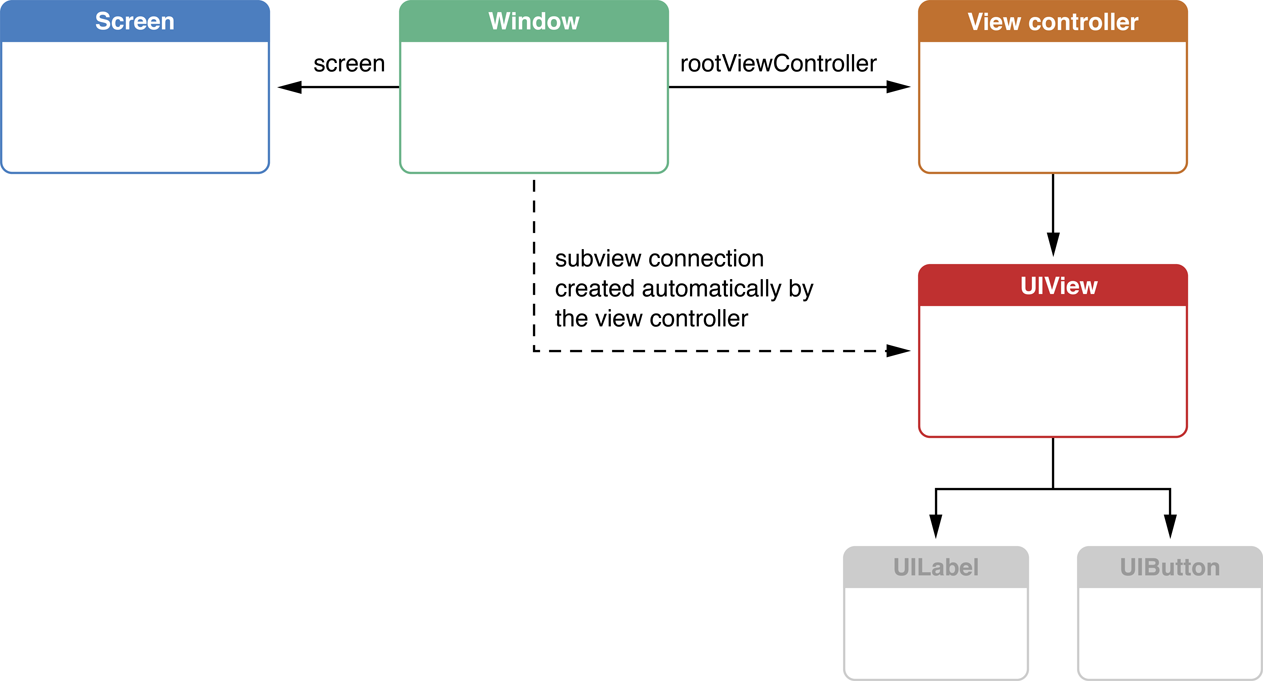
\includegraphics[totalheight=0.35\textheight]{../figuras/ios/apple_window_view_controller_screen.png}
  \caption{Esquema relacionando os elementos da UI}
  \label{fig:a}
\end{figure}

\bigskip

\subsection{UIView x UIViewController}

\paragraph{}Um objeto do tipo UIView, ou apenas \emph{View}, é onde colocamos de fato os elementos visuais. Ela representa uma determinada área onde pode conter objetos como UIButton, UILabel e UITextField, além de outras \emph{Views} inseridas, formando uma hierarquia de objetos que vão se orientar diretamente pelo posicionamento e comportamento da UIView maior.
\paragraph{}A grande ideia a ser entendida e que diferencia uma \emph{View} de uma \emph{View Controller} é que um objeto de UIView contém estritamente elementros gráficos, sem nenhuma lógica do comportamento. Um objeto de UIView não entende e não deve entender as consequências de suas ações. Um UIButton, por exemplo, sabe como agir quando é clicado mas não sabe qual tipo de ação ou mensagem foi gerada e nem pra onde ela foi a partir do seu clique.
\paragraph{}Deixando algumas coisas claras, uma tela pode conter uma só \emph{View} tomando todo o espaço ou várias \emph{Views} se divindido, sendo elas totalmente independentes ou aninhadas. Além disso, você pode criar novas classes herdando de UIView para serem estanciadas dentro de uma UIViewController.\\

\paragraph{}Uma \emph{View Controller} é o que gerencia a lógica e comportamento de um conjunto específico de uma ou mais \emph{Views}, e é responsável por carregar e interagir com as \emph{Views} na hora correta e da forma correta. Um UIButton clicado envia um sinal para a \emph{View Controller}, que tem o papel de entender qual deve ser a resposta para esse evento, que pode ser algo como envio de dados, interação com as \emph{Views}, ou criação de animações.
\paragraph{}Uma \emph{View Controller} é criada com uma única \emph{View} atrelada. É possível então adicionar mais \emph{Views} dentro da \emph{View} principal ou em conjunto com ela.
\paragraph{}Sabendo que é possível criar uma classe para uma \emph{View} genérica, sem possuir uma \emph{View Controller} atrelada, como sabemos se criamos uma classe herdando de UIView ou de UIViewController? Essa pergunta pode causar confusão no início, mas fica mais claro após entender exatamente o papel de cada uma.
\paragraph{}Primeiramente seguimos a regra de que para cada tela completa criamos uma \emph{View Controller} para gerenciá-la, e nessa classe podemos inserir todos os elementos da tela. Porém há os casos em que a ideia é criar uma \emph{View} genérica a ser inserida no contexto de uma tela completa, \emph{View} essa que pode ser desde uma célula customizada para uma tabela até uma tabela completa, aí então devemos pensar se essa mesma \emph{View} terá algum comportamento ou se será unicamente visual. No caso de uma célula customizada, por exemplo, ela será apenas visual e assim deve ser uma simples classe de UIView; já no caso de uma tabela completa, ela vai precisar de um grande conjunto de lógica para o seu comportamento, portanto precisará de uma \emph{View Controller} própria, que no caso de tabelas tem uma classe especial chamada UITableViewController.

\bigskip

\subsection{Navegação entre telas}

\bigskip

\begin{figure}[h]
  \centering
  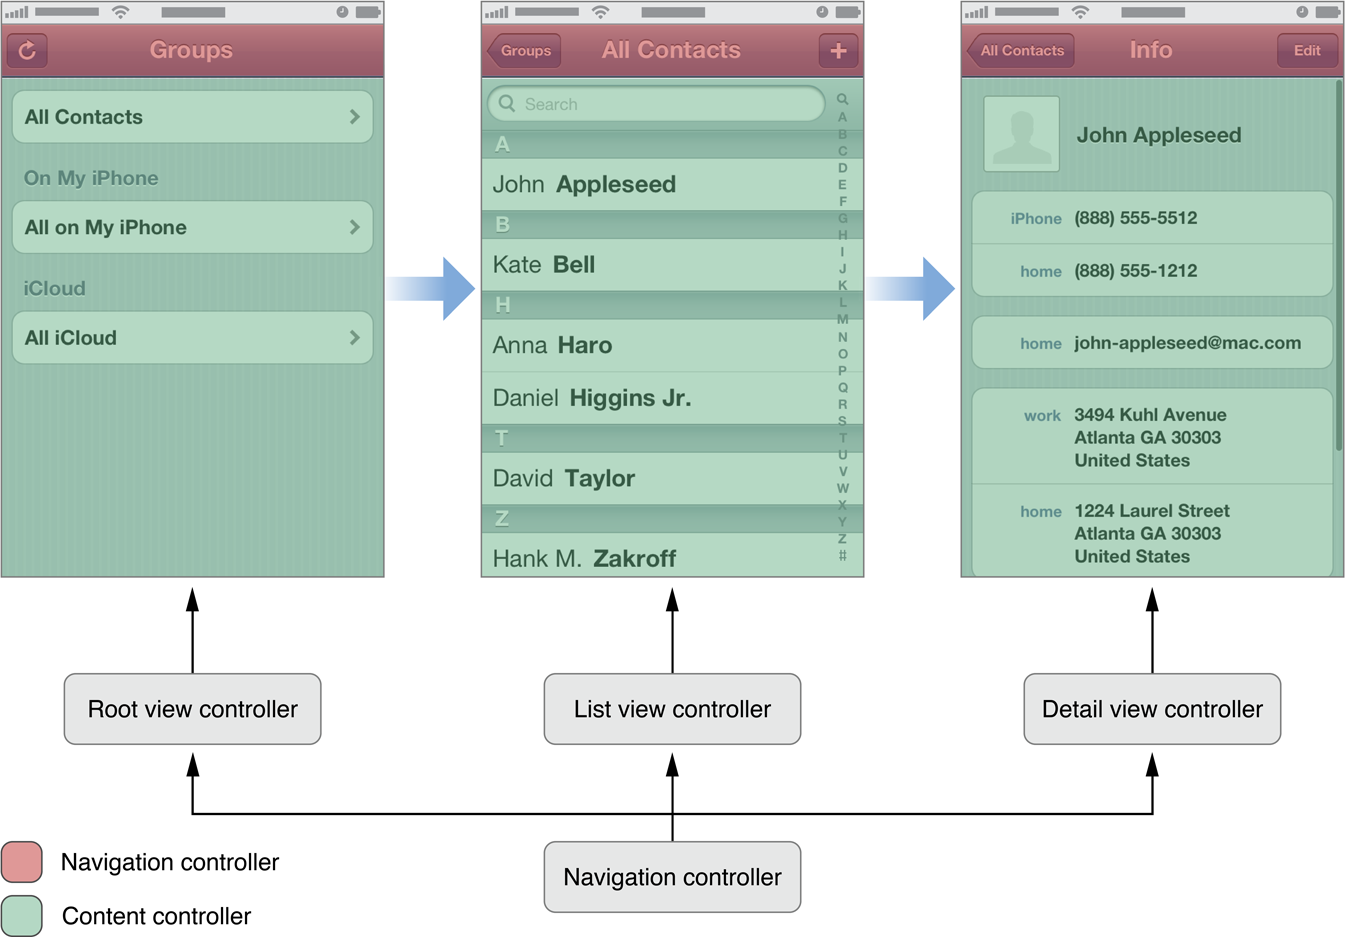
\includegraphics[totalheight=0.35\textheight]{../figuras/ios/apple_navigation_interface.png}
  \caption{Esquema do funcionamento do Navigation Controller}
  \label{fig:a}
\end{figure}

\bigskip

\paragraph{}Conforme vamos criando novas telas, precisamos de um modo de chamá-las e de retornar delas para a tela anterior. O iOS permite mais de um tipo de gerenciamento de navegação das telas, mas em quase 100\% dos casos faremos uso do \emph{Navigation Controller}.
\paragraph{}O \emph{Navigation Controller} funciona como uma pilha de \emph{View Controllers} que tem início sempre na já citada \emph{Root View Controller}, que será a tela inicial do aplicativo. Definimos uma única vez pelo código qual será nossa \emph{Root View Controller}, após isso trabalharemos apenas com métodos de \emph{push} e \emph{pop} para carregar e descarregar as telas. Graficamente, o \emph{Navigation Controller} é a barra superior (que também pode ser inferior) nas telas dos aplicativos e que contém um botão de retorno e outros botões auxiliares.
\paragraph{}Há um outro tipo de navegação complementar chamado \emph{Tab Bar Controller}, que nada mais é que uma nova tela, que pode inclusive estar contida na pilha do \emph{Navigation Controller}, e que traz duas ou mais telas divididas por abas.

\bigskip

\begin{figure}[h]
  \centering
  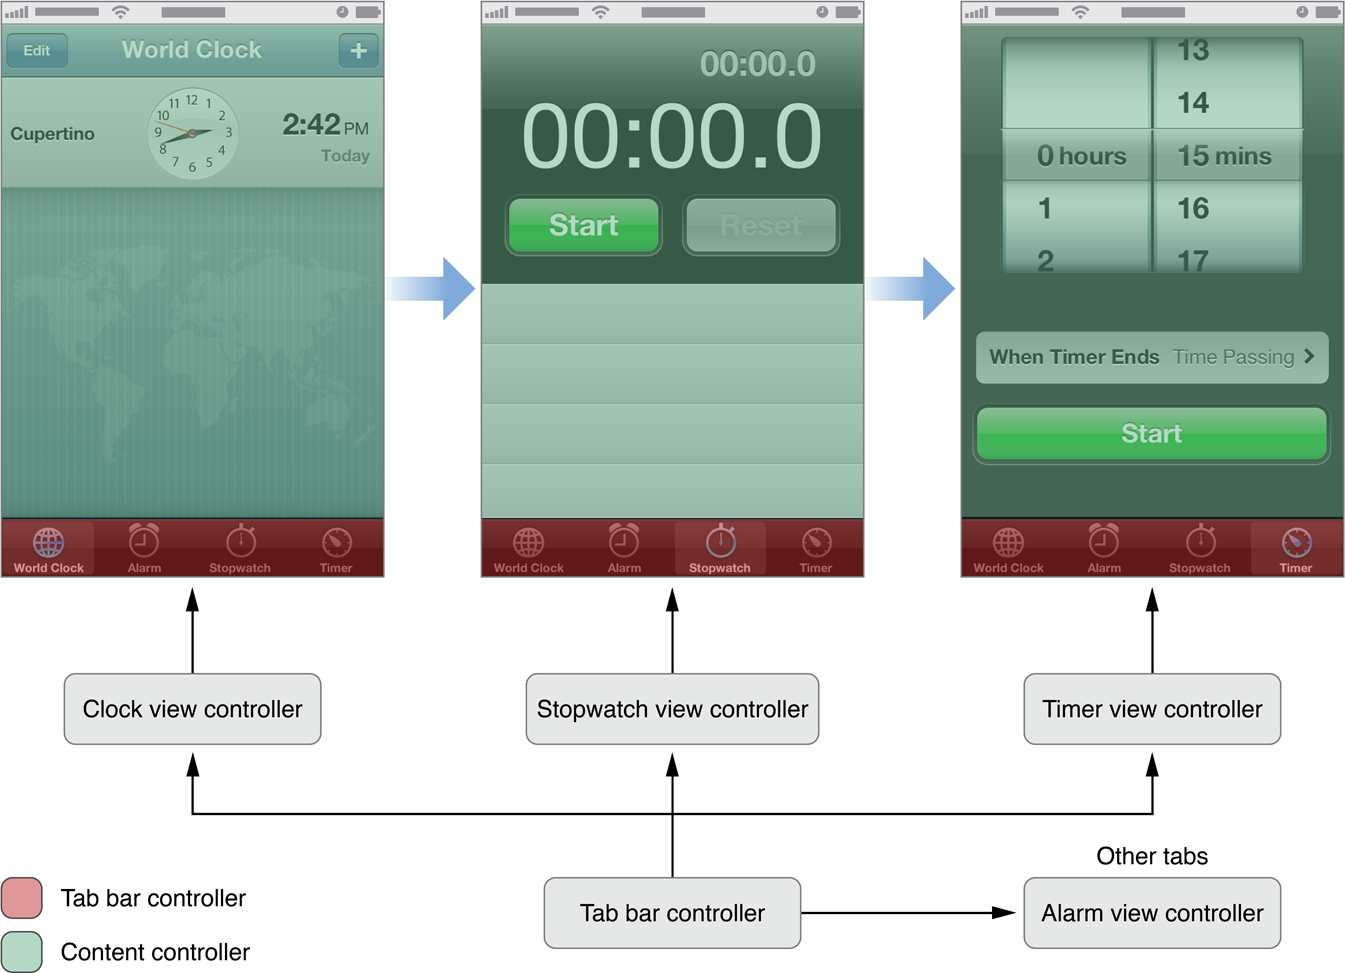
\includegraphics[totalheight=0.4\textheight]{../figuras/ios/apple_tabbar_interface.png}
  \caption{Esquema do funcionamento do Tab Bar Controller}
  \label{fig:a}
\end{figure}

\bigskip
\bigskip


\section{Interface Builder}

\paragraph{}Para nos auxiliar na construção das telas, utilizeremos o Interface Builder do XCode. Na criação de uma nova \emph{View Controller}, é criado um arquivo *.xib atrelado a essa classe, que ligará automaticamente os objetos criados na interface ao código da classe.
\paragraph{}O Interface Builder é uma ferramente muito poderosa e o utilizaremos principalmente para definir o posicionamento dos objetos, como as \emph{Views} e seus componentes, e para fazer a ligação dos \emph{outlets} e \emph{actions} ao código.
\paragraph{}E lembrando que sempre podemos determinar o layout e a criação dos objetos diretamente no código, sendo o Interface Builder apenas um facilitador. Em diversos casos lidar com o código acaba sendo até mais prático.

\bigskip

\subsection{Outlets e Actions}

\paragraph{}\emph{Outlets} representam uma ligação entre um objeto criado na interface pelo Interface Builder, como um botão ou um texto, e uma instância criada no código. Funciona como um ponteiro de um objeto do código para a sua representação gráfica, e assim podemos nos referenciar a esse elemento no código do \emph{View Controller} para definirmos seu comportamento e possíveis mudanças nas suas características.
\paragraph{}Já uma \emph{action} representa uma mensagem enviada por um objeto na interface. A \emph{action} define o tipo de toque que aciona a mensagem e cria o método que será chamado e conterá o código do programador para definir o comportamento desejado.

\bigskip
\bigskip


\section{Seu primeiro aplicativo}

\paragraph{}Agora vamos enfim colocar a mão na massa e colocar em ordem tudo que foi falado até agora.

\bigskip

\subsection{Primeira tela}

\subsection{Ligando novas telas}

\subsection{Trocando informação}

\subsection{O uso do Delegate}

\thispagestyle{empty}

\doublespace
%\onehalfspace
%\singlespace

\cleardoublepage

\pagestyle{body}
\pagenumbering{arabic}


\begin{singlespace}

\lstinputlisting[float, language=java, label=cod:exemplo, caption={Exemplo ... \citep{muchnick}}]{../../src/android/teste.java}

\end{singlespace}


%%%%%%%%%%%%%%%%%%%%%%%%%%%%%%%%%%%%%%%%%%%%%%%%%%%%%%%%%%%%%%%%%%%%%%%%%%%%%%%%

\singlespace
\selectlanguage{brazil}
\cleardoublepage
\thispagestyle{empty}
\phantomsection
\addcontentsline{toc}{chapter}{Referências Bibliográficas}
\bibliography{../comum/biblio}
\bibliographystyle{apalike}
\doublespace


\appendix
\addtocontents{toc}{\protect\setcounter{tocdepth}{0}} % as seções do apêndice não aparecem do sumário com este comando...
%%%%%%%%%%%%%%%%%%%%%%%%%%%%%%%%%%%%%%%%%%%%%%%%%%%%%%%%%%%%%%%%%%%%%%%%%%%%%%%%
\ape{apen}{Especificação blá, blá, blá}

Isto é um apêndice...

%%%%%%%%%%%%%%%%%%%%%%%%%%%%%%%%%%%%%%%%%%%%%%%%%%%%%%%%%%%%%%%%%%%%%%%%%%%%%%%%
\addtocontents{toc}{\protect\setcounter{tocdepth}{1}}

\end{document}
